\documentclass[article]{jss}
\usepackage{thumbpdf} 
\graphicspath{{Figures/}}

\usepackage{acronym}
\usepackage{cleveref}
\usepackage{subfig}
\usepackage{framed}

\acrodef{CRAN}[CRAN]{Comprehensive \proglang{R} Archive Network}
\acrodef{mlp}[MLP]{multilayer perceptron}
\acrodef{nid}[NID]{neural interpretation diagram}

\crefname{figure}{Figure}{Figures}

\author{Marcus W. Beck\\US Environmental Protection Agency}

\title{\pkg{NeuralNetTools}: Visualization and Analysis Tools for Neural Networks}

\Plainauthor{Marcus W. Beck} 
\Plaintitle{NeuralNetTools: Visualization and Analysis Tools for Neural Networks}

\Shorttitle{\pkg{NeuralNetTools}: Visualization and Analysis Tools for Neural Networks} 

\Abstract{ Supervised neural networks have been applied as a machine
  learning technique to identify and predict emergent patterns among
  multiple variables.  A common criticism of these methods is the
  inability to characterize relationships among variables from a
  fitted model. Although several techniques have been proposed to
  ``illuminate the black box'', they have not been made available in an
  open-source programming environment.  This article describes the
  \pkg{NeuralNetTools} package that can be used for the interpretation
  of supervised neural network models created in \proglang{R}.
  Functions in the package can be used to visualize a model using a
  neural network interpretation diagram, evaluate variable importance
  by disaggregating the model weights, and perform a sensitivity
  analysis of the response variables to changes in the input
  variables.  Methods are provided for objects from many of the common
  neural network packages in \proglang{R}, including \pkg{caret},
  \pkg{neuralnet}, \pkg{nnet}, and \pkg{RSNNS}.  The article provides
  a brief overview of the theoretical foundation of neural networks, a
  description of the package structure and functions, and an applied
  example to provide a context for model development with
  \pkg{NeuralNetTools}.  Overall, the package provides a toolset for
  neural networks that complements existing quantitative techniques
  for data-intensive exploration.  }

\Keywords{neural networks, \code{plotnet}, sensitivity, variable
  importance, \proglang{R}}

\Plainkeywords{neural networks, plotnet, sensitivity, variable
  importance, R}

%% \Volume{50}
%% \Issue{9}
%% \Month{June}
%% \Year{2012}
%% \Submitdate{2012-06-04}
%% \Acceptdate{2012-06-04}

\Address{
  Marcus W. Beck\\
  US Environmental Protection Agency\\
  National Health and Environmental Effects Research Laboratory\\
  Gulf Ecology Division, 1 Sabine Island Drive\\
  Gulf Breeze, Florida, 32561, USA\\
  \textit{Current address:} Southern California Coastal Water Research Project\\
  3535 Harbor Blvd., Suite 110\\
  Costa Mesa, CA, 92626\\
  Telephone: +1/714/755/3217\\
  E-mail: \email{marcusb@sccwrp.org}
}

\begin{document}

\section[Introduction]{Introduction}

A common objective of data-intensive analysis is the synthesis of
unstructured information to identify patterns or trends ``born from the
data'' \citep{Bell09,Kelling09,Michener12}.  Analysis is primarily
focused on data exploration and prediction as compared to
hypothesis-testing using domain-specific methods for scientific
exploration \citep{Kell03}.  Demand for quantitative toolsets to
address challenges in data-rich environments has increased drastically
with the advancement of techniques for rapid acquisition of
data. Fields of research characterized by high-throughput data (e.g.,
bioinformatics; \citealt{Saeys07}) have a strong foundation in
computationally-intensive methods of analysis, whereas disciplines
that have historically been limited by data quantity (e.g., field
ecology; \citealt{Swanson15}) have also realized the importance of
quantitative toolsets given the development of novel techniques to
acquire information.  Quantitative methods that facilitate inductive
reasoning can serve a complementary role to conventional,
hypothesis-driven approaches to scientific discovery \citep{Kell03}.

Statistical methods that have been used to support data exploration
are numerous \citep{Jain00,Recknagel06,Zuur10}.  A common theme among
data intensive methods is the use of machine-learning algorithms where
the primary objective is to identify emergent patterns with minimal
human intervention.  Neural networks, in particular, are designed to
mimic the neuronal structure of the human brain by ``learning'' inherent
data structures through adaptive algorithms
\citep{Rumelhart86,Ripley96}.  Although the conceptual model was
introduced several decades ago \citep{McCulloch43}, neural networks
have had a central role in emerging fields focused on data
exploration.  The most popular form of neural network is the
feed-forward \ac{mlp} trained using the backpropagation algorithm
\citep{Rumelhart86}.  This model is typically used to predict the
response of one or more variables given one to many explanatory
variables.  The hallmark feature of the \ac{mlp} is the
characterization of relationships using an arbitrary number of
parameters (i.e., the hidden layer) that are chosen through iterative
training with the backpropagation algorithm.  Conceptually, the
\ac{mlp} is a hyper-parameterized non-linear model that can fit a
smooth function to any dataset with minimal residual error
\citep{Hornik91}.

An arbitrarily large number of parameters to fit a neural network
provides obvious predictive advantages, but complicates the extraction
of model information.  Diagnostic information such as variable
importance or model sensitivity are necessary aspects of exploratory
data analysis that are not easily obtained from a neural network. As
such, a common criticism is that neural networks are ``black boxes''
that offer minimal insight into relationships among variables
\citep[e.g.,][]{Paruelo97}.  \citet{Olden02} provide a rebuttal to
this concern by describing methods to extract information about
variable relationships from neural networks.  Many of these methods
were previously described but not commonly used.  For example,
\citet{Olden02} describe the \ac{nid} for plotting \citep{Ozesmi99},
the Garson algorithm for variable importance \citep{Garson91}, and the
profile method for sensitivity analysis \citep{Lek96}.  These
quantitative tools ``illuminate the black box'' by disaggregating the
network parameters to characterize relationships between variables
that are described by the model.  Although \ac{mlp} neural networks
were developed for prediction, methods described in \citet{Olden02}
leverage these models to describe data signals.  Increasing the
accessibility of these diagnostic tools will have value for exploratory
data analysis and may also inform causal inference.

This article describes the \pkg{NeuralNetTools} package
\citep{NeuralNetTools} for \proglang{R} \citep{R} that was developed
to better understand information obtained from the \ac{mlp} neural
network.  Functions provided by the package are those described in
\citet{Olden02} but have not been previously available in an
open-source programming environment.  The reach of the package is
extensive in that generic functions were developed for model objects
from the most popular neural network packages available in
\proglang{R}.  The objectives of this article are to 1) provide an
overview of the statistical foundation of the \ac{mlp} network, 2)
describe the theory and application of the main functions in the
\pkg{NeuralNetTools} package, and 3) provide an applied example using
neural networks and \pkg{NeuralNetTools} in data exploration.  The
current released package version is available from the \ac{CRAN}
(CRAN) at \url{https://CRAN.R-project.org/package=NeuralNetTools},
whereas the development version is maintained as a GitHub repository.

\section[Theoretical foundation and existing R packages]{Theoretical foundation and existing \proglang{R} packages}

The typical \ac{mlp} network is composed of multiple layers that
define the transfer of information between input and response layers.
Information travels in one direction where a set of values for
variables in the input layer propagates through one or more hidden
layers to the final layer of the response variables. Hidden layers
between the input and response layers are key components of a neural
network that mediate the transfer of information.  Just as the input
and response layers are composed of variables or nodes, each hidden
layer is composed of nodes with weighted connections that define the
strength of information flow between layers.  Bias layers connected to
hidden and response layers may also be used that are analogous to
intercept terms in a standard regression model.

Training a neural network model requires identifying the optimal
weights that define the connections between the model layers.  The
optimal weights are those that minimize prediction error for a test
dataset that is independent of the training dataset.  Training is
commonly achieved using the backpropagation algorithm described in
\citet{Rumelhart86}.  This algorithm identifies the optimal weighting
scheme through an iterative process where weights are gradually
changed through a forward- and backward-propagation process
\citep{Rumelhart86,Lek00}.  The algorithm begins by assigning an
arbitrary weighting scheme to the connections in the network, followed
by estimating the output in the response variable through the
forward-propagation of information through the network, and finally
calculating the difference between the predicted and actual value of
the response.  The weights are then changed through a backpropagation
step that begins by changing weights in the output layer and then the
remaining hidden layers.  The process is repeated until the chosen
error function is minimized, as in standard model-fitting techniques
for regression \citep{Cheng94}.  A fitted \ac{mlp} neural network can
be represented as \citep{Bishop95,Venables02}:
\begin{equation}
y_k = f_o \left(\sum\limits_{h} w_{hk}f_h \left( \sum\limits_{i} w_{ih}x_i\right) \right),
\end{equation}
where the estimated value of the response variable $y_k$ is a sum of
products between the respective weights $w$ for $i$ input variables
$x$ and $h$ hidden nodes, mediated by the activation functions $f_h$
and $f_o$ for each hidden and output node.

Methods in \pkg{NeuralNetTools} were written for several \proglang{R}
packages that can be used to create \ac{mlp} neural networks:
\pkg{neuralnet} \citep{Fritsch12}, \pkg{nnet} \citep{Venables02}, and
\pkg{RSNNS} \citep{Bergmeir12}. Limited methods were also developed
for neural network objects created with the \code{train} function from
the \pkg{caret} package \citep{Kuhn15}.  Additional \proglang{R}
packages that can create \ac{mlp} neural networks include \pkg{AMORE}
that implements the ``TAO-robust backpropagation algorithm'' for model
fitting \citep{Castejon14}, \pkg{FCNN4R} that provides an \proglang{R}
interface to the \pkg{FCNN} \proglang{C++} library \citep{Klima15},
\pkg{monmlp} for networks with partial monotonicity constraints
\citep{Cannon15}, and \pkg{qrnn} for quantile regression neural
networks \citep{Cannon11}.  At the time of writing, the \ac{CRAN}
download logs \citep{Csardi15} showed that the \proglang{R} packages
with methods in \pkg{NeuralNetTools} included 95\% of all downloads
for the available \ac{mlp} packages, with \pkg{nnet} accounting for
over 78\%.  As such, methods have not been included in
\pkg{NeuralNetTools} for the remaining packages, although further
development of \pkg{NeuralNetTools} could include additional methods
based on popularity.  Methods for each function are currently
available for `\code{mlp}' (\pkg{RSNNS}), `\code{nn}'
(\pkg{neuralnet}), `\code{nnet}' (\pkg{nnet}), and `\code{train}'
(\pkg{caret}; only if the object also inherits from the `\code{nnet}'
class) objects.  Additional default methods or methods for class
`\code{numeric}' are available for some of the generic functions.

\section[Package structure]{Package structure}

The stable release of \pkg{NeuralNetTools} can be installed from \ac{CRAN} and loaded as follows:
%
\begin{Schunk}
\begin{Sinput}
R> install.packages("NeuralNetTools")
R> library("NeuralNetTools")
\end{Sinput}
\end{Schunk}
%
\pkg{NeuralNetTools} includes four main functions that were developed
following similar techniques in \citet{Olden02} and references
therein.  The functions include \code{plotnet} to plot a neural
network interpretation diagram, \code{garson} and \code{olden} to
evaluate variable importance, and \code{lekprofile} for a sensitivity
analysis of neural network response to input variables.  Most of the
functions require the extraction of model weights in a common format
for the neural network object classes in \proglang{R}.  The
\code{neuralweights} function can be used to retrieve model weights
for any of the model classes described above.  A two-element
\code{list} is returned with the first element describing the
structure of the network (number of nodes in the input, hidden, and
output layers) and the second element as a named list of model
weights.  The function is used internally within the main functions
but may also be useful for comparing networks of different classes.

A common approach for data pre-processing is to normalize the input
variables and to standardize the response variables
\citep{Lek00,Olden02}.  A sample dataset that follows this format is
included with \pkg{NeuralNetTools}.  The \code{neuraldat} dataset is a
simple \code{data.frame} with 2000 rows of observations and five
columns for two response variables (\code{Y1} and \code{Y2}) and three
input variables (\code{X1}, \code{X2}, and \code{X3}).  The input
variables are random observations from a standard normal distribution
and the response variables are linear combinations of the input
variables with additional random components.  The response variables
are also scaled from zero to one.  Variables in additional datasets can be
pre-processed to this common format using the \code{scale} function
from \pkg{base} to center and scale input variables (i.e., z-scores) 
and the \code{rescale} function from \pkg{scales} to scale response variables 
from zero to one.  The examples below use three models created from the 
\code{neuraldat} dataset and include `\code{mlp}' (\pkg{RSNNS}), `\code{nn}' 
(\pkg{RSNNS}), and `\code{nnet}' (\pkg{nnet}) objects.
%
\begin{Schunk}
\begin{Sinput}
R> set.seed(123)
R> library("RSNNS")
R> x <- neuraldat[, c("X1", "X2", "X3")]
R> y <- neuraldat[, "Y1"]
R> mod1 <- mlp(x, y, size = 5)
R> library("neuralnet")
R> mod2 <- neuralnet(Y1 ~ X1 + X2 + X3, data = neuraldat, hidden = 5)
R> library("nnet")
R> mod3 <- nnet(Y1 ~ X1 + X2 + X3, data = neuraldat, size = 5)
\end{Sinput}
\end{Schunk}

\subsection{Visualizing neural networks}

Existing plot functions in \proglang{R} to view neural networks are
minimal.  Such tools have practical use for visualizing network
architecture and connections between layers that mediate variable
importance. To our knowledge, only the \pkg{neuralnet} and
\pkg{FCNN4R} packages provide plotting methods for \ac{mlp} networks
in \proglang{R}.  Although useful for viewing the basic structure, the
output is minimal and does not include extensive options for
customization.

The \code{plotnet} function in \pkg{NeuralNetTools} plots a \acl{nid}
\citep[\acs{nid};][]{Ozesmi99} and includes several options to
customize aesthetics. A \ac{nid} is a modification of the standard
conceptual illustration of the \ac{mlp} network that changes the
thickness and color of the weight connections based on magnitude and
sign, respectively.  Positive weights between layers are shown as
black lines and negative weights as gray lines. Line thickness is
proportional to the absolute magnitude of each weight
(\cref{fig:plotnet}).

\begin{figure}[t!]
\subfloat[][]{
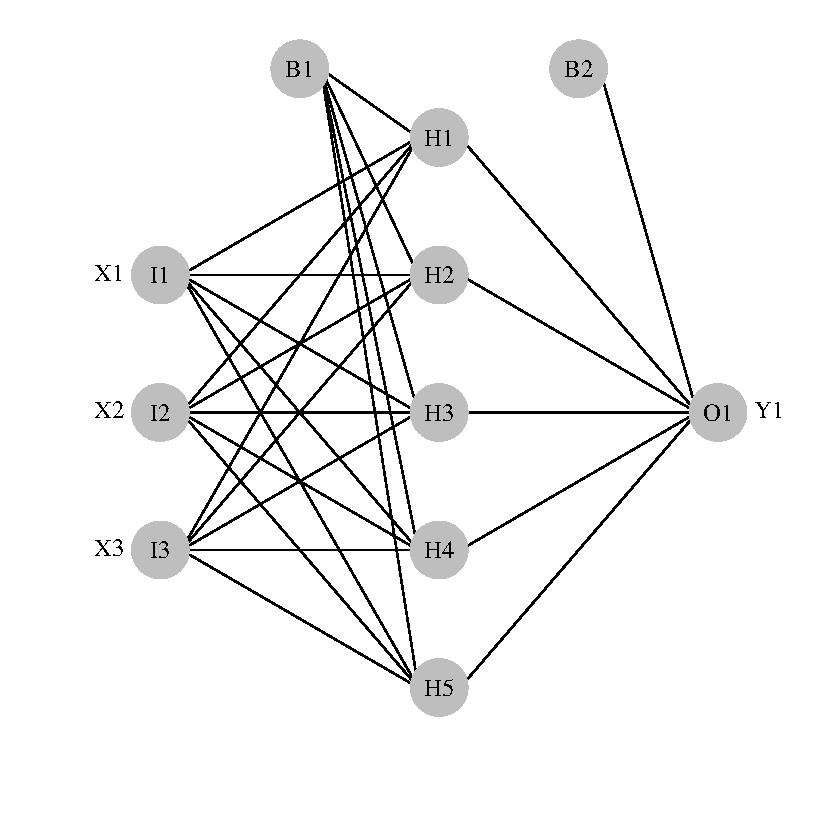
\includegraphics[width=7.5cm,page=1, trim = 0 20 0 15, clip]{plotnet.pdf}
\label{fig:plotnet1}
}
\subfloat[][]{
\includegraphics[width=7.5cm, page=2, trim = 0 20 0 15, clip]{plotnet.pdf}
\label{fig:plotnet2}
}
\caption{Examples from the \code{plotnet} function showing neural networks as a standard graphic (\ref{fig:plotnet1}) and using the \acl{nid} (\ref{fig:plotnet2}).  Labels outside of the nodes represent variable names and labels within the nodes indicate the layer and node (I: input, H: hidden, O: output, B: bias).}
\label{fig:plotnet}
\end{figure}

A primary and skip layer network can also be plotted for `\code{nnet}'
models with a skip layer connection (\cref{fig:plotnet_skip}). Models
with skip layers include additional connections from the input to
output layers that bypass the hidden layer \citep{Ripley96}.  The
default behavior of \code{plotnet} is to plot the primary network,
whereas the skip layer can be viewed separately with \code{skip =
  TRUE}. If \code{nid = TRUE}, the line widths for both the primary
and skip layer plots are relative to all weights. Plotting a network
with only a skip layer (i.e., no hidden layer, \code{size = 0} in
\code{nnet}) will include bias connections to the output layer,
whereas these are included only in the primary plot if size is greater
than zero.

\begin{figure}[t!]
\subfloat[][]{
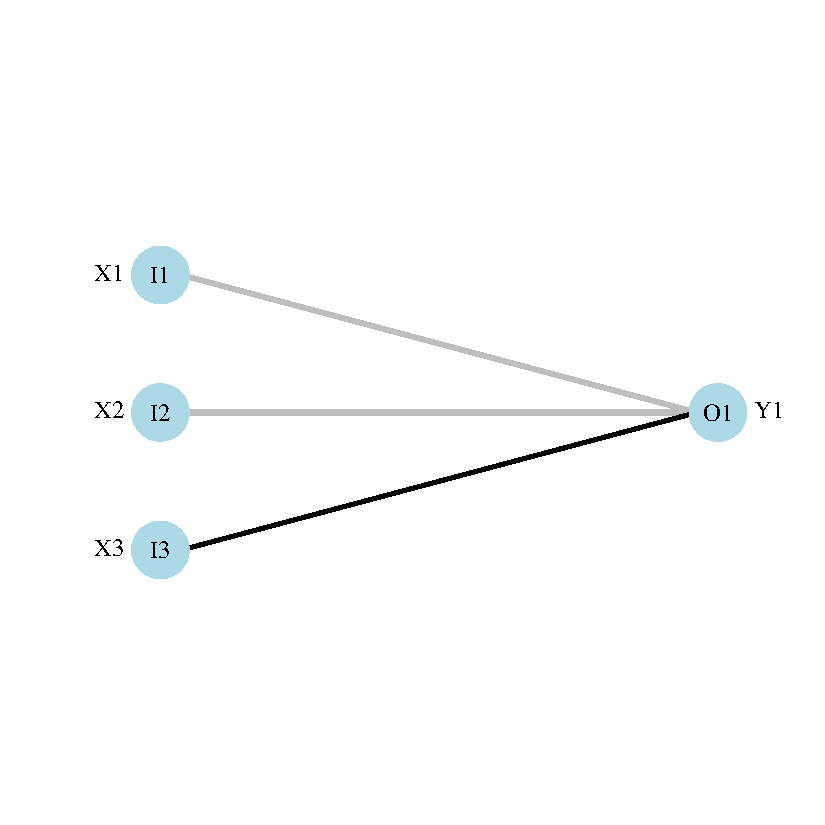
\includegraphics[width=7.5cm,page=1, trim = 0 20 0 15, clip]{plotnet_skip.pdf}
\label{fig:plotnet_skip1}
}
\subfloat[][]{
\includegraphics[width=7.5cm, page=2, trim = 0 20 0 15, clip]{plotnet_skip.pdf}
\label{fig:plotnet_skip2}
}
\caption{Examples from the \code{plotnet} function showing a neural network with a separate skip layer between the input and output layers.  The skip layer (\ref{fig:plotnet_skip1}) and primary neural network (\ref{fig:plotnet_skip2}) can be viewed separately with \code{plotnet} by using \code{skip = TRUE} or \code{skip = FALSE}.}
\label{fig:plotnet_skip}
\end{figure}

The \pkg{RSNNS} package provides algorithms to prune connections or
nodes in a neural network \citep{Bergmeir12}.  This approach can
remove connection weights between layers or input nodes that do not
contribute to the predictive performance of the network.  In addition
to visualizing connections in the network that are not important,
connections that are pruned can be removed in successive model
fitting.  This reduces the number of free parameters (weights) that
are estimated by the model optimization algorithm, increasing the
likelihood of convergence to an estimable numeric solution for the
remaining connection weights that minimizes prediction error
\citep[i.e., model identifiability;][]{Ellenius00}. Algorithms in
\pkg{RSNNS} for weight pruning include magnitude-based pruning,
optimal brain damage, and optimal brain surgeon, whereas algorithms
for node pruning include skeletonization and the non-contributing
units method \citep{Zell98}.  The \code{plotnet} function can plot a
pruned neural network, with options to omit or display the pruned
connections (\cref{fig:plotprune}).
%
\begin{Schunk}
\begin{Sinput}
R> pruneFuncParams <- list(max_pr_error_increase = 10.0,
+    pr_accepted_error = 1.0, no_of_pr_retrain_cycles = 1000, 
+    min_error_to_stop = 0.01, init_matrix_value = 1e-6,  
+    input_pruning = TRUE, hidden_pruning = TRUE)
R> mod <- mlp(x, y, size = 5, pruneFunc = "OptimalBrainSurgeon",
+    pruneFuncParams = pruneFuncParams)
R> plotnet(mod, rel_rsc = c(3, 8))
R> plotnet(mod, prune_col = "lightblue", rel_rsc = c(3, 8))
\end{Sinput}
\end{Schunk}
%
Note that the pruned network obtained with \pkg{RSNNS} and thus this
plot might vary depending on the platform used.
%
\begin{figure}[t!]
\subfloat[][]{
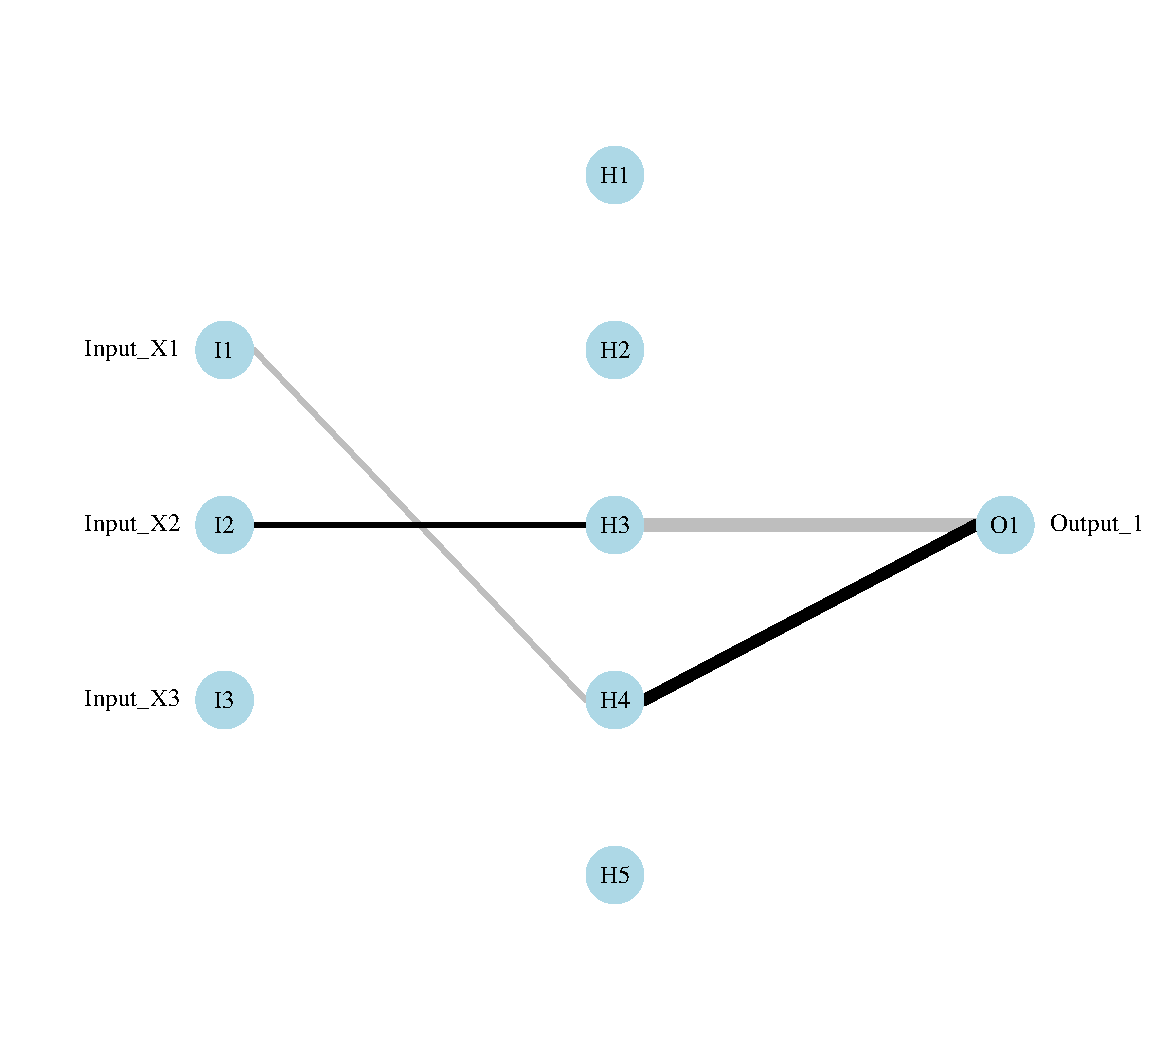
\includegraphics[width=0.48\textwidth, page=1, trim = 0 20 0 65, clip]{plotprune.pdf}
\label{fig:plotprune1}
}
\subfloat[][]{
\includegraphics[width=0.48\textwidth, page=2, trim = 0 20 0 65, clip]{plotprune.pdf}
\label{fig:plotprune2}
}
\caption{A pruned neural network from \pkg{RSNNS} \citep{Bergmeir12}
  using the ``optimal brain surgeon'' algorithm described in
  \citet{Zell98}.  The default plotting behavior of \code{plotnet} is
  to omit pruned connections (\ref{fig:plotprune1}), whereas they can
  be viewed as dashed lines by including the \code{prune\_col}
  argument (\ref{fig:plotprune2}).}
\label{fig:plotprune}
\end{figure}

\subsection{Evaluating variable importance}

The primary benefit of visualizing a \ac{nid} with \code{plotnet} is the ability to evaluate network architecture and the variation in connections between the layers.  Although useful as a general tool, the \ac{nid} can be difficult to interpret given the amount of weighted connections in most networks.  Alternative methods to quantitatively describe a neural network deconstruct the model weights to determine variable importance, whereas similar information can only be qualitatively inferred from \code{plotnet}.  Two algorithms for evaluating variable importance are available in \pkg{NeuralNetTools}: Garson's algorithm for relative importance \citep{Garson91,Goh95} and Olden's connection weights algorithm \citep{Olden04}.

Garson's algorithm was originally described by \citet{Garson91} and further modified by \citet{Goh95}.  The \code{garson} function is an implementation of the method described in the appendix of \citet{Goh95} that identifies the relative importance of each variable as an absolute magnitude. For each input node, all weights connecting an input through the hidden layer to the response variable are identified to return a list of all weights specific to each input variable. Summed products of the connections for each input node are then scaled relative to all other inputs. A value for each input node indicates relative importance as the absolute magnitude from zero to one. The method is limited in that the direction of the response cannot be determined and only neural networks with one hidden layer and one output node can be evaluated.

The \code{olden} function is a more flexible approach to evaluate variable importance using the connection weights algorithm \citep{Olden04}. This method calculates importance as the summed product of the raw input-hidden and hidden-output connection weights between each input and output node. An advantage is the relative contributions of each connection weight are maintained in both magnitude and sign. For example, connection weights that change sign (e.g., positive to negative) between the input-hidden to hidden-output layers would have a canceling effect, whereas \code{garson} may provide different results based on the absolute magnitude. An additional advantage is that the \code{olden} function can evaluate neural networks with multiple hidden layers and response variables. The importance values assigned to each variable are also in units based on the summed product of the connection weights, whereas \code{garson} returns importance scaled from 0 to 1.

Both functions have similar implementations and require only a model
object as input.  The default output is a \pkg{ggplot2} bar plot
\citep[i.e., \code{geom\_bar};][]{Wickham09} that shows the relative
importance of each input variable in the model (\cref{fig:plotimp}).
The plot aesthetics are based on internal code that can be changed
using conventional syntax for \pkg{ggplot2} applied to the output
object.  The importance values can also be returned as a
\code{data.frame} if \code{bar\_plot = FALSE}.  Variable importance
shown in \Cref{fig:plotimp} is estimated for each model using:
%
\begin{Schunk}
\begin{Sinput}
R> garson(mod1)
R> olden(mod1)
R> garson(mod2)
R> olden(mod2)
R> garson(mod3)
R> olden(mod3)
\end{Sinput}
\end{Schunk}
%
\begin{figure}[t!]
\centering
\subfloat[][Model 1 (`\code{mlp}'), \code{garson}]{
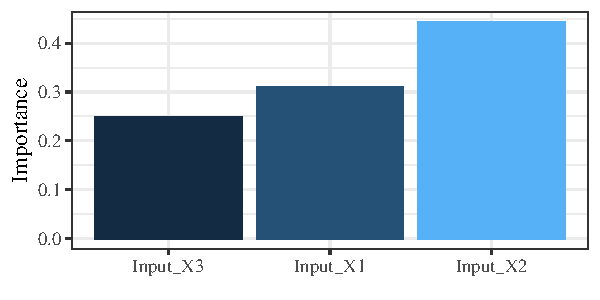
\includegraphics[width = 0.47\textwidth, page = 1]{plotimp.pdf}
\label{fig:plotimp1}
}
\subfloat[][Model 1 (`\code{mlp}'), \code{olden}]{
\includegraphics[width = 0.47\textwidth, page = 2]{plotimp.pdf}
\label{fig:plotimp2}
}

\subfloat[][Model 2 (`\code{nn}'), \code{garson}]{
\includegraphics[width = 0.47\textwidth, page = 3]{plotimp.pdf}
\label{fig:plotimp3}
}
\subfloat[][Model 2 (`\code{nn}'), \code{olden}]{
\includegraphics[width = 0.47\textwidth, page = 4]{plotimp.pdf}
\label{fig:plotimp4}
}

\subfloat[][Model 3 (`\code{nnet}'), \code{garson}]{
\includegraphics[width = 0.47\textwidth, page = 5]{plotimp.pdf}
\label{fig:plotimp5}
}
\subfloat[][Model 3 (`\code{nnet}'), \code{olden}]{
\includegraphics[width = 0.47\textwidth, page = 6]{plotimp.pdf}
\label{fig:plotimp6}
}
\caption{Variable importance for three models using Garson's algorithm
  for relative importance (\code{garson},
  \cref{fig:plotimp1,fig:plotimp3,fig:plotimp5};
  \citealt{Garson91,Goh95}) and Olden's connection weights algorithm
  (\code{olden}, \cref{fig:plotimp2,fig:plotimp4,fig:plotimp6};
  \citealt{Olden04}).  Garson's algorithm shows importance as absolute
  values from 0--1, whereas Olden's algorithm preserves sign and
  magnitude.  Importance values for Olden's algorithm are from the
  summed product of model weights and are not rescaled.}
\label{fig:plotimp}
\end{figure}

\subsection{Sensitivity analysis}

An alternative approach to evaluate variable relationships in a neural
network is the Lek profile method \citep{Lek96,Gevrey03}. The profile
method differs fundamentally from the variable importance algorithms
by evaluating the behavior of response variables across different
values of the input variables. The method is generic and can be
extended to any statistical model in \proglang{R} with a
\code{predict} method. However, it is one of few methods used to
evaluate sensitivity in neural networks.

The \code{lekprofile} function evaluates the effects of input
variables by returning a plot of model predictions across the range of
values for each variable.  The remaining explanatory variables are
held constant when evaluating the effects of each input variable.  The
\code{lekprofile} function provides two options for setting constant
values of unevaluated explanatory variables.  The first option follows
the original profile method by holding unevaluated variables at
different quantiles (e.g., minimum, 20th percentile, maximum;
\cref{fig:plotlek_sens1,fig:plotlek_bars1}). This is implemented by
creating a matrix where the number of rows is the number of
observations in the original dataset and the number of columns is the
number of explanatory variables. All explanatory variables are held
constant (e.g., at the median) while the variable of interest is
sequenced from its minimum to maximum. This matrix is then used to
predict values of the response variable from a fitted model
object. This is repeated for each explanatory variable to obtain all
response curves.  Constant values are set in \code{lekprofile} by
passing one or more values in the range 0--1 to the \code{group\_vals}
argument.  The default holds variables at the minimum, 20th, 40th,
60th, 80th, and maximum percentiles (i.e., \code{group\_vals = c(0,
  0.2, 0.4, 0.6, 0.8, 1)}).

A second implementation of \code{lekprofile} is to group the
unevaluated explanatory variables by natural groupings defined by the
data. Covariance among predictors may present unlikely scenarios if
all unevaluated variables are held at the same level (e.g., high
values for one variable may be unlikely with high values for a second
variable). The second option holds unevaluated variables at means
defined by natural clusters in the data
(\cref{fig:plotlek_sens2,fig:plotlek_bars2}). Clusters are identified
using {\it k}-means clustering (\code{kmeans} from the base package
\pkg{stats}; \citealt{Hartigan79}) of the input variables if the
argument passed to \code{group_vals} is an integer greater than
one. The centers (means) of the clusters are then used as constants
for the unevaluated variables.  \citet{Beck14a} provide an example of
the clustering method for \code{lekprofile} by evaluating response of
a lake health index to different explanatory variables.  Lake clusters
were identified given covariance among variables, such that holding
explanatory variables at values defined by clusters created more
interpretable response curves.  Both methods return similar plots,
with additional options to visualize the groupings for unevaluated
explanatory variables (\cref{fig:plotlek_bars}).  For the latter case,
\code{group\_show = TRUE} will return a stacked bar plot for each
group with heights within each bar proportional to the constant
values.  Sensitivity profiles were created using the standard approach
based on quantiles and using the alternative clustering method
(\cref{fig:plotlek_sens}), including bar plots of the relative values
for unevaluated explanatory variables (\cref{fig:plotlek_bars}).
%
\begin{Schunk}
\begin{Sinput}
R> lekprofile(mod3)
R> lekprofile(mod3, group_show = TRUE)
R> lekprofile(mod3, group_vals = 6)
R> lekprofile(mod3, group_vals = 6, group_show = TRUE)
\end{Sinput}
\end{Schunk}
%
\begin{figure}[t!]
\centering
\subfloat[][Response with quantiles]{
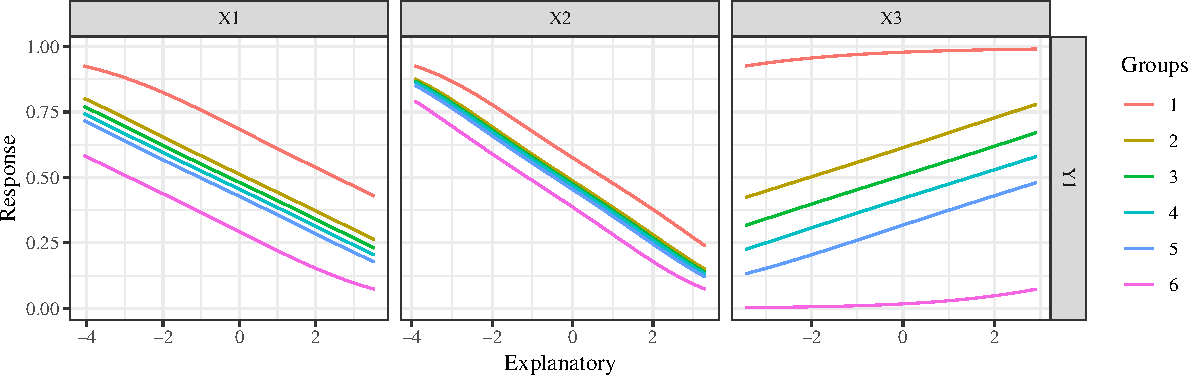
\includegraphics[width = 0.9\textwidth, page = 1]{plotlek_sens.pdf}
\label{fig:plotlek_sens1}
}

\subfloat[][Response with clusters]{
\includegraphics[width = 0.9\textwidth, page = 2]{plotlek_sens.pdf}
\label{fig:plotlek_sens2}
}
\caption{Sensitivity analysis of a neural network using the Lek profile method to evaluate the effects of explanatory variables.  \Cref{fig:plotlek_sens1} groups unevaluated explanatory variables at quantiles (minimum, 20th, 40th, 60th, 80th, and maximum percentiles) and \cref{fig:plotlek_sens2} groups by cluster means (six groups).  Values at which explanatory variables are held constant for each group are shown in \cref{fig:plotlek_bars1,fig:plotlek_bars2}.}
\label{fig:plotlek_sens}
\end{figure}

%%%%
\begin{figure}[t!]  
\centering
\subfloat[][Quantile groupings]{
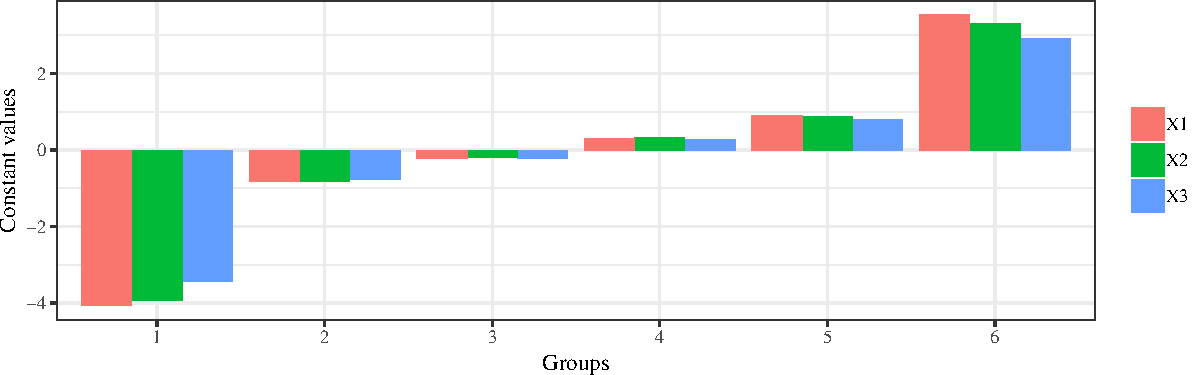
\includegraphics[width = 0.9\textwidth, page = 1]{plotlek_bars.pdf}
\label{fig:plotlek_bars1}
}

\subfloat[][Cluster groupings]{
\includegraphics[width = 0.9\textwidth, page = 2]{plotlek_bars.pdf}
\label{fig:plotlek_bars2}
}
\caption{Bar plots for values of unevaluated explanatory variables in each group in \cref{fig:plotlek_sens1,fig:plotlek_sens2}.  \Cref{fig:plotlek_bars1} shows default quantile groupings set at the minimum, 20th, 40th, 60th, 80th, and maximum percentiles.  For example, variables are held at negative values for group~1 (i.e., stacked bars with negative heights) for the minimum value, whereas group~6 holds variables at their maximum (largest positive heights). \Cref{fig:plotlek_bars2} shows the cluster centers for each variable in each group.  Groups in \cref{fig:plotlek_bars2} are random because the input variables are from a standard normal distribution.}
\label{fig:plotlek_bars}
\end{figure}

\section[Applied example]{Applied example}

Although \pkg{NeuralnetTools} provides several methods to extract
information from a fitted neural network, it does not provide explicit
guidance for developing the initial model.  A potentially more
challenging aspect of using \ac{mlp} neural networks is understanding
the effects of network architecture on model performance, appropriate
use of training and validation datasets, and implications for the
bias-variance tradeoff with model over- or under-fitting
\citep{Maier00}.  A detailed discussion of these issues is beyond the
scope of this paper, although an example application is presented
below to emphasize the importance of these considerations.  The models
presented above, including the \code{neuraldat} dataset, are contrived
examples to illustrate use of the \pkg{NeuralNetTools} package and
they do not demonstrate a comprehensive or practical application of
model development.  In general, the following should be considered
during initial development \citep{Ripley96, Lek00, Maier00}:
\begin{itemize}
\item Initial data pre-processing to normalize inputs, standardize response, and assess influence of outliers.
\item Network architecture including number of hidden layers, number of nodes in each hidden layer, inclusion of bias or skip layers, and pruning weights or inputs.
\item Separating data into training and test datasets, e.g., 2:1, 3:1, leave-one-out, etc.
\item Initial starting weights for the backpropagation algorithm.
\item Criteria for stopping model training, e.g., error convergence tolerance, maximum number of iterations, minimum error on test dataset, etc.
\end{itemize}

A dataset from \pkg{nycflights13} \citep{Wickham14b} is used to
demonstrate (1) the use of the functions in \pkg{NeuralNetTools} to
gain additional insight into relationships among variables, and (2)
the effects of training conditions on model conclusions.
This dataset provides information on all flights departing New York
City (i.e., JFK, LGA, or EWR) in 2013.  The example uses all flights
from the UA carrier in the month of December to identify variables
that potentially influence arrival delays (\code{arr\_delay}, minutes)
at the destination airport.  Factors potentially related to delays
are selected from the dataset and include departure delay
(\code{dep\_delay}, minutes), departure time (\code{dep\_time}, hours,
minutes), arrival time (\code{arr\_time}, hours, minutes), travel time
between destinations (\code{air\_time}, minutes), and distance flown
(\code{distance}, miles).

First, the appropriate month and airline carrier are selected, all
explanatory variables are scaled and centered, and the response variable is
scaled to 0--1.
%
\begin{Schunk}
\begin{Sinput}
R> library("nycflights13")
R> library("dplyr")
R> tomod <- filter(flights, month == 12 & carrier == "UA") %>% 
+    select(arr_delay, dep_delay, dep_time, arr_time, air_time,
+      distance) %>% mutate_each(funs(scale), -arr_delay) %>% 
+    mutate_each(funs(as.numeric), -arr_delay) %>% 
+    mutate(arr_delay = scales::rescale(arr_delay, to = c(0, 1))) %>% 
+    data.frame
\end{Sinput}
\end{Schunk}
%
Then, a standard MLP with five hidden nodes was created with the
\pkg{nnet} package to model the effects of selected variables on
arrival delays. The entire dataset is used for the example but
separate training and validation datasets should be used in practice.
%
\begin{Schunk}
\begin{Sinput}
R> library("nnet")
R> mod <- nnet(arr_delay ~ ., size = 5, linout = TRUE, data = tomod,
+    trace = FALSE)  
\end{Sinput}
\end{Schunk}
%
The default output is limited to structural information about the model and methods for model predictions (see \code{str(mod)} and \code{?predict.nnet}). Using functions from \pkg{NeuralNetTools}, a more comprehensive understanding of the relationships between the variables is illustrated.
%
\begin{Schunk}
\begin{Sinput}
R> plotnet(mod)
R> garson(mod)
R> olden(mod)
R> lekprofile(mod, group_vals = 5)
R> lekprofile(mod, group_vals = 5, group_show = TRUE)
\end{Sinput}
\end{Schunk}
%
\Cref{fig:flightplots} shows the information about arrival delays that
can be obtained with the functions in \pkg{NeuralNetTools}. The
\ac{nid} (\ref{fig:flightplotsa}) shows the model structure and can be
used as a general characterization of the relationships between
variables.  For example, most of the connection weights from input
nodes I2 and I5 are strongly negative (gray), suggesting that departure 
time and distance traveled has an opposing relationship with arrival 
delays. Similarly, large positive weights are observed for I3 and I4, 
suggesting arrival time and time in the air are positively associated 
with arrival delays.  However, interpreting individual connection weights 
between layers is challenging. Figures~\ref{fig:flightplotsb} and 
\ref{fig:flightplotsc} provide more quantitative descriptions using 
information from both the \ac{nid} and model predictions.  
\Cref{fig:flightplotsb} shows variable importance using the \code{garson} 
and \code{olden} algorithms.  The \code{garson} function suggests time 
between destinations (\code{air\_time}) has the strongest relationship 
with arrival delays, similar to a strong positive association shown 
with the \code{olden} method. However, the \code{garson} function 
shows arrival time (\code{arr\_time}) as the third most important 
variable for arrival delays, whereas this is ranked highest by the \code{olden}
function. Similar discrepancies between the two methods are observed
for other variables, which are explained below. Finally, results from
the \code{lekprofile} function (Figure~\ref{fig:flightplotsc}) confirm those
in Figure~\ref{fig:flightplotsb}, with the addition of non-linear responses
that vary by different groupings of the data.  Values for each
variable in the different unevaluated groups (based on clustering)
show that there were no obvious patterns between groups, with the
exception being group one that generally had longer times in the air 
and greater distance travelled.

%%%%
\begin{figure}[t!]
\centering
\subfloat[][\code{plotnet}]{
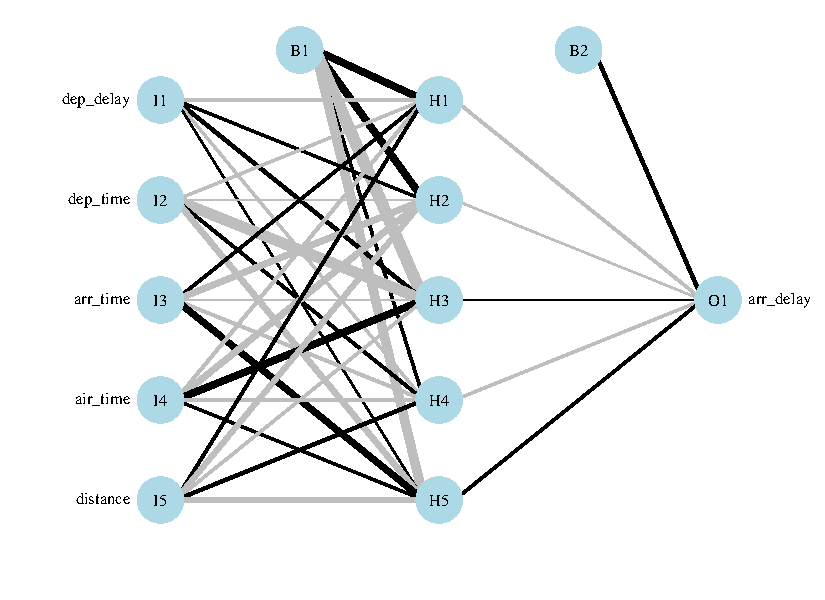
\includegraphics[width = 0.5\textwidth, page = 1]{flightplots1.pdf}
\label{fig:flightplotsa}
}
\subfloat[][\code{garson} (top) and \code{olden} (bottom)]{
\includegraphics[width = 0.5\textwidth, page = 2]{flightplots1.pdf}
\label{fig:flightplotsb}
}

\subfloat[][\code{lekprofile}]{
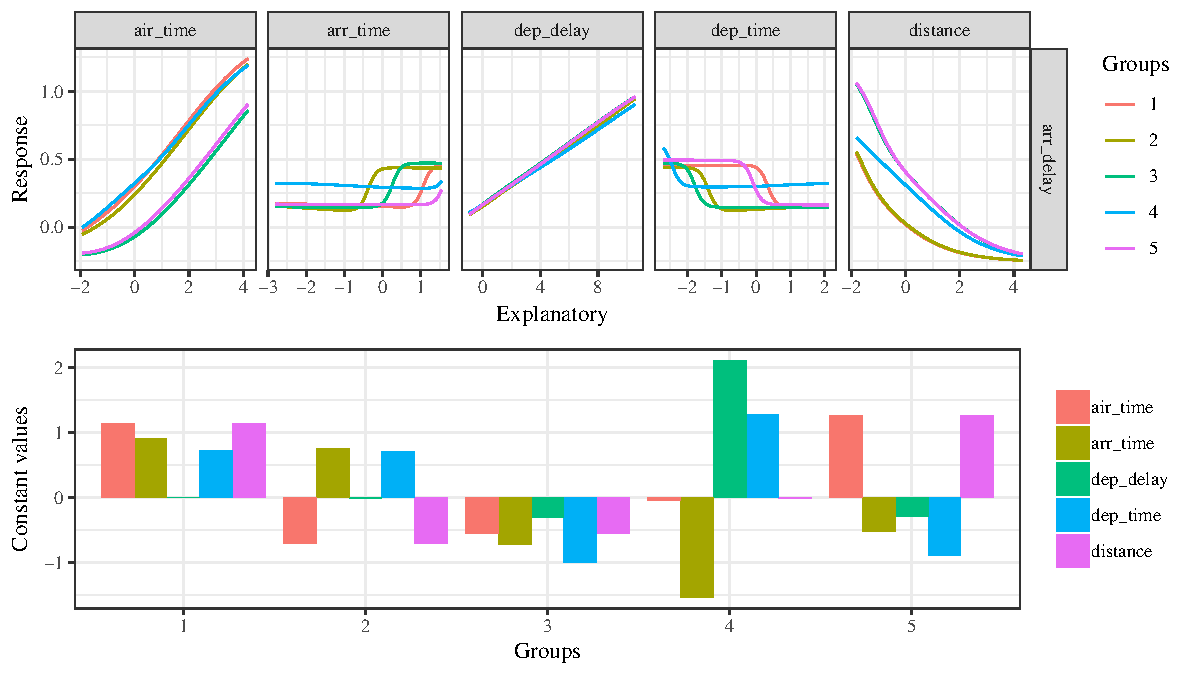
\includegraphics[width = 1.05\textwidth, page = 1]{flightplots2.pdf}
\label{fig:flightplotsc}
}

\caption{Results from a simple \ac{mlp} model of arrival delay for December airline flights versus departure delay (\code{dep\_delay}), departure time (\code{dep\_time}), arrival time (\code{arr\_time}), travel time between destinations (\code{air\_time}), and distance flown (\code{distance}). The three plots show the \ac{nid} from \code{plotnet} (\ref{fig:flightplotsa}), variable importance with \code{garson} and \code{olden} (\ref{fig:flightplotsb}), and sensitivity analysis with variable groupings from \code{lekprofile} (\ref{fig:flightplotsc}). Interpretations are provided in the text.}
\label{fig:flightplots}
\end{figure}

A second analysis is needed to show the effects of network
architecture and initial starting weights on uncertainty in estimates
of variable importance. Models with one, five, or ten hidden nodes and
100 separate models for each node level are created.  Each model has
a random set of starting weights for the first training iteration.
Importance estimates using \code{olden} are saved for each model and
combined in a single plot to show overall variable importance as the
median and 5th/95th percentiles from the 100 models for each node
level.

Several conclusions from \cref{fig:flightimp} provide further
information to interpret the trends in \cref{fig:flightplots}.  First,
consistent relationships can be identified such that delays in arrival
time are negatively related to distance and positively related to
departure delays and air time.  That is, flights arrived later than
their scheduled time if flight time was long or if their departure was
delayed, whereas flights arrived earlier than scheduled for longer
distances.  No conclusions can be made for the other variables because
the bounds of uncertainty include zero.  Second, the range of
importance estimates varies between the models (i.e., one node varies
between $\pm 1$ and the others between $\pm 3$).  This suggests that
the relative importance estimates only have relevance within each
model, whereas only the rankings (e.g., least, most important) can be
compared between models.  Third and most important, the level of
uncertainty for specific variables can be large between model fits for
the same architecture.  This suggests that a single model can provide
misleading information and therefore several models may be required to
decrease uncertainty.  Additional considerations described above
(e.g., criteria for stopping training, use of training and test
datasets) can also affect the interpretation of model information and
should be considered equally during model development.
\begin{figure}[t!]
\centering
\subfloat[][Networks with one node]{
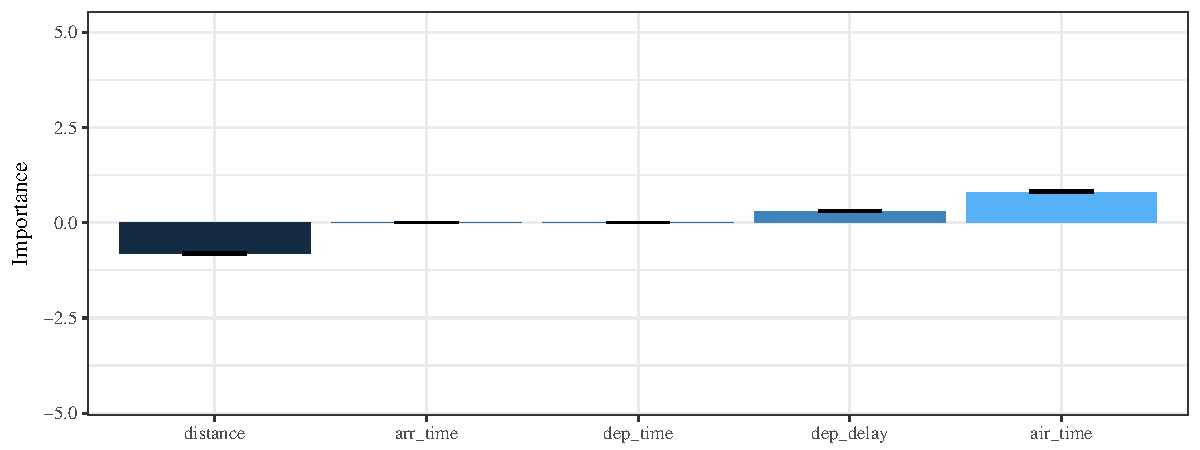
\includegraphics[width = 0.95\textwidth, page = 1]{flightimp.pdf}
\label{fig:flightimp1}
}

\subfloat[][Networks with five nodes]{
\includegraphics[width = 0.95\textwidth, page = 2]{flightimp.pdf}
\label{fig:flightimp2}
}

\subfloat[][Networks with ten nodes]{
\includegraphics[width = 0.95\textwidth, page = 3]{flightimp.pdf}
\label{fig:flightimp3}
}
\caption{Uncertainty in variable importance estimates for three neural networks to evaluate factors related to arrival delays for flights departing New York City.  Three model types with one, five, and ten nodes were evaluated with 100 models with different starting weights for each type.}
\label{fig:flightimp}
\end{figure}

\section[Conclusions]{Conclusions}

The \pkg{NeuralNetTools} package provides a simple approach to improve
the quality of information obtained from a feed-forward \ac{mlp}
neural network.  Functions can be used to visualize a neural network
using a \acl{nid} (\code{plotnet}), evaluate variable importance
(\code{garson}, \code{olden}), and conduct a sensitivity analysis
(\code{lekprofile}).  Although visualizing a neural network with
\code{plotnet} is impractical for large models, the remaining
functions can simplify model complexity to identify important
relationships between variables.  Methods are available for the most
frequently used \ac{CRAN} packages that can create neural networks
(\pkg{caret}, \pkg{neuralnet}, \pkg{nnet}, \pkg{RSNNS}), whereas
additional methods could be added based on popularity of the remaining
packages (\pkg{AMORE}, \pkg{FCNN4R}, \pkg{monmlp}, \pkg{qrnn}).

A primary objective of the package is to address the concern that
supervised neural networks are ``black boxes'' that provide no
information about underlying relationships between variables
\citep{Paruelo97,Olden02}.  Although neural networks are considered
relatively complex statistical models, the theoretical foundation has
many parallels with simpler statistical techniques that provide for
evaluation of variable importance \citep{Cheng94}.  Moreover, the model
fitting process minimizes error using a standard objective function
such that conventional techniques to evaluate model sensitivity or
performance (e.g., cross-validation) can be used with neural networks.
As such, functions in \pkg{NeuralNetTools} can facilitate the
selection of the optimal network architecture or can be used for
post-hoc assessment.

Another important issue is determining when and how to apply neural
networks given availability of alternative methods of analysis.  The
popularity of the \ac{mlp} neural network is partly to blame for the
generalizations and misperceptions about their benefits as modeling
tools \citep{Burke97}. Perhaps an overstatement, the neural component
is commonly advertised as a mathematical representation of the network
of synaptic impulses in the human brain.  Additionally, several
examples have shown that the \ac{mlp} network may provide comparable
predictive performance as similar statistical methods
\citep{Feng02,Razi05,Beck14a}.  A neural network should be considered
a tool in the larger toolbox of data-intensive methods that should be
used after examination of the tradeoffs between techniques, with
particular emphasis on the specific needs of a dataset or research
question.  Considerations for choosing a method may include power
given the sample size, expected linear or non-linear interactions
between variables, distributional forms of the response, and other
relevant considerations of exploratory data analysis \citep{Zuur10}.
\pkg{NeuralNetTools} provides analysis tools that can inform
evaluation and selection from among several alternative methods for
exploratory data analysis.

\section*{Acknowledgments}
 
I thank Bruce Vondracek, Sanford Weisberg, and Bruce Wilson of the
University of Minnesota for general guidance during the development of
this package.  Thanks to Sehan Lee and Marc Weber for reviewing an
earlier draft.  Contributions and suggestions from online users have
also greatly improved the utility of the package.  Funding for this
project was supported in part by an Interdisciplinary Doctoral
Fellowship provided by the Graduate School at the University of
Minnesota to M.~Beck.

\bibliography{ref}

\end{document}
